\chapter{Direct Dialling}
\label{ch:DirectDialling}

\section{Introduction}
\label{sec:DDIntro}
This chapter serves as a good introduction to some of the important concepts
that will crop up later on. I will begin with an introduction to the Reck
scheme \cite{reck94}, an architecture for realising any unitary matrix in linear
optics; then proceed to explain \bosonsampling{} \cite{bosonsampling}, a task
that may enable a demonstration of computational superiority of linear optics
over classical computers. The main results of the chapter concerns the important
task of dialling Haar random unitary matrices into a linear-optical Reck scheme.
This is achieved by way of a coordinate transformation parameterising unitaries
in terms of physical parameters. The final section is a further application of
this parameterisation to the task of inferring the unitary description of a
linear optical circuit.

\section{A universal circuit for linear optics}
\label{sec:ReckScheme}
Any lossless\footnote{In practical devices, this approximation is very good.
\todo{1dB/cm in silica devices?}} linear optical device can be
described by a unitary matrix operating on the optical modes. A device with
\(m\) input and \(m\) output modes will be described by an \(m \by m\) unitary.
In~\cite{reck94}, it is shown that the converse is true: any unitary matrix can
be realised by a linear optical circuit. A constructive proof of this is
presented, and a candidate `universal circuit' is proposed. Universal, in this
context refers to a linear optical circuit with adjustable components
(beamsplitters with variable reflectivity and variable phase shifts), which can
be configured into any unitary.

\begin{figure}
  \begin{subfigure}{\textwidth}
    \centering
    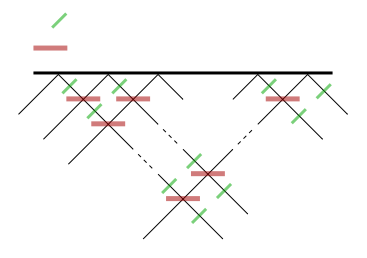
\includegraphics{figures/reck_original}
    \caption{The original Reck scheme, implemented in bulk optics. As with all
    circuits in bulk optics, achieving phase stability in this system would be
    very difficult.}
    \label{fig:ReckOriginal}
  \end{subfigure} \\
  \vspace{1cm} \\
  \begin{subfigure}{\textwidth}
    \centering
    \includegraphics{figures/reck_general}
    \caption{A more modern take on the Reck scheme. Here we envisage using
    a triangular array of
    Mach-Zehnder interferometers (MZIs) on an integrated platform, thus solving
    the phase stability problem.}
    \label{fig:ReckGeneral}
  \end{subfigure}
  \caption[The Reck scheme, in both its original conception and an integrated
  optics version]{The Reck scheme, in both its original conception and an
  integrated
  optics version. In both systems, light enters from the left and the device
  performs a unitary transformation on the modes. Variable-reflectivity
  beamsplitters and variable phase shifts are needed in order to make the
  circuit's operation reconfigurable to any unitary transformation. In the
  bulk scheme, I have omitted any specifics, but in the integrated version these
  could be implemented with directional couplers and thermal or electro-optic
  phase shifts \todo{citation needed}.}
  \label{fig:ReckScheme}
\end{figure}

\section{Boson Sampling}
\label{sec:BosenSampling}
This section presents a review of \bosonsampling{}: a sampling algorithm
presented by Aaronson and Arkhipov in~\cite{bosonsampling}. None of development
or complexity analysis of this algorithm is my own work, but it provides useful
context for the material later in this chapter.

\section{Dialling Haar unitaries}
\label{sec:Parameterization}
Now for the main result of this chapter: how do we dial a Haar random unitary in
a linear optical device. Given a unitary matrix, there is a straightforward
algorithm \todo{is this presented in Reck?} to extract the appropriate circuit
parameters, and this method applies as well to random matrices as any others.
Here I describe a method which bypasses the generation of the matrix, instead
operating directly on the circuit parameters. I derive probability density
functions for each component in the Reck scheme and present a proof that
choosing parameters independently from these pdfs will result in Haar random
unitary matrices.

\begin{figure}
  \begin{subfigure}{0.43\textwidth}
    \centering
    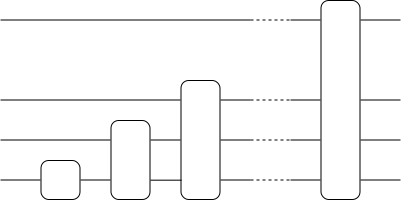
\includegraphics{figures/reck_schematic}
    \caption{}
    \label{fig:ReckSchematic}
  \end{subfigure}
  \hspace{0.04\textwidth}
  \begin{subfigure}{0.53\textwidth}
    \centering
    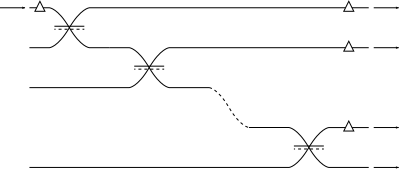
\includegraphics{figures/cascade}
    \caption{}
    \label{fig:Cascade}
  \end{subfigure}
  \caption[The Reck scheme in terms of successive operations on vectors]
  {The Reck scheme in terms of successive operations on vectors}
  \label{fig:ReckCascade}
\end{figure}

At the heart of the proof is a coordinate transformation between the Cartesian
basis (i.e. the numbers that we write down in a matrix) and the physical basis
(the values of beamsplitter reflectivities and phase shifts in the physical
realisation of the unitary.

\section{Unitary Inference}
\label{sec:UnitaryInference}
One of the most important tasks in practical quantum computing is that of
tomography: what does the device in the lab actually do? Although general
methods exist \todo{citation needed}, they are intractable, requiring a number
of measurements that scales exponentially in system size.
